\documentclass[a4paper,11pt]{article}
\usepackage{amssymb}
\usepackage[polish]{babel}
\usepackage[utf8]{inputenc}
\usepackage[T1]{fontenc}
\usepackage{array}
\usepackage{graphicx}
\usepackage{anysize}
\usepackage{enumerate}
\usepackage{times}
\usepackage{geometry}
\usepackage{amsthm}
\usepackage{pgfplots}
\usepackage{sidecap}
\usepackage{wrapfig}
\usepackage[format=hang,font=small,labelfont=bf]{caption}
\usepackage[intlimits]{amsmath}
\marginsize{3cm}{3cm}{1.5cm}{1.5cm}
\sloppy

\begin{document}
\begin{table}[ht]
\centering
\hspace*{-1cm}
\begin{tabular}{lllllll}
\cline{1-6}
\multicolumn{1}{|c|}{\begin{tabular}[c]{@{}c@{}}EAIiIB\\ Informatyka\end{tabular}}              & \multicolumn{2}{l|}{\begin{tabular}[c]{@{}l@{}}Ewa Stachów\\ Weronika Olcha\end{tabular}}                                                                                                & \multicolumn{1}{c|}{\begin{tabular}[c]{@{}c@{}}Rok\\ II\end{tabular}}          & \multicolumn{1}{c|}{\begin{tabular}[c]{@{}c@{}}Grupa\\ 3\end{tabular}}            & \multicolumn{1}{c|}{\begin{tabular}[c]{@{}c@{}}Zespół\\ 6\end{tabular}}      &  \\ \cline{1-6}
\multicolumn{1}{|c|}{\begin{tabular}[c]{@{}c@{}}Pracownia\\ FIZYCZNA\\ WFiIS AGH\end{tabular}} & \multicolumn{4}{l|}{\begin{tabular}[c]{@{}l@{}}Temat:\\ \textbf{\textit{Opracowanie danych pomiarowych}} \end{tabular}}                                                                                                                                                                                                                                            & \multicolumn{1}{c|}{\begin{tabular}[c]{@{}c@{}}Nr ćwiczenia:\\ 0\end{tabular}} &  \\ \cline{1-6}
\multicolumn{1}{|l|}{\begin{tabular}[c]{@{}c@{}}Data wykonania:\\ 7.10.2016\end{tabular}}      & \multicolumn{1}{c|}{\begin{tabular}[c]{@{}c@{}}Data oddania:\\ 12.10.2016\end{tabular}} & \multicolumn{1}{l|}{\begin{tabular}[c]{@{}l@{}}Zwrot do poprawki:\\ \phantom{data poprawki}\end{tabular}} & \multicolumn{1}{l|}{\begin{tabular}[c]{@{}l@{}}Data oddania:\\  \phantom{data oddania}\end{tabular}} & \multicolumn{1}{l|}{\begin{tabular}[c]{@{}l@{}}Data zaliczenia:\\  \phantom{data zaliczenia}\end{tabular}} & \multicolumn{1}{l|}{\begin{tabular}[c]{@{}l@{}}OCENA:\\ \phantom{ocena}\end{tabular}}       &  \\ \cline{1-6}                                                                                           
\end{tabular}
\hspace*{-1cm}
\end{table}

\begin{center}
\begin{LARGE}
\textbf{Ćwiczenie nr 0: Opracowanie danych pomiarowych}
\end{LARGE}
\end{center}

\section{Cel ćwiczenia}

Zaznajomienie się z typowymi metodami opracowania danych pomiarowych przy wykorzystaniu wyników pomiarów dla wahadła prostego. 

\section{Wstęp teoretyczny}
\begin{wrapfigure}{l}{0.25\textwidth}
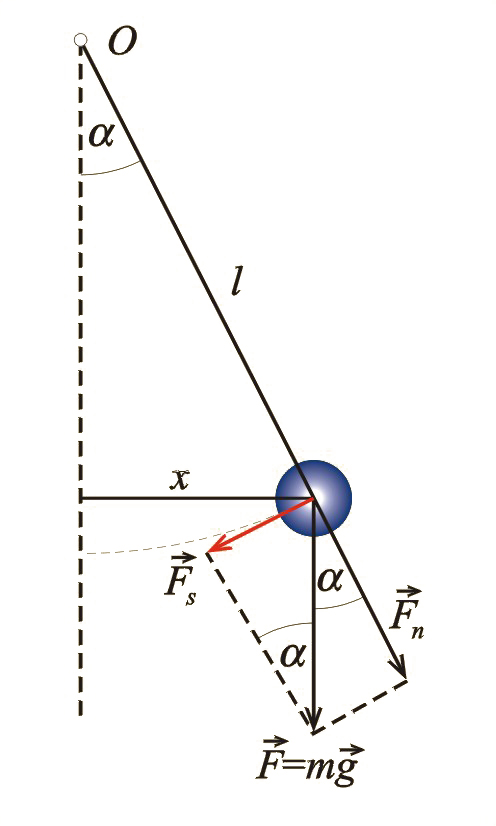
\includegraphics[width=0.25\textwidth]{./wahadlowstep}
\end{wrapfigure}
Wahadło matematyczne to punkt materialny zawieszony na nieważkiej i nierozciągliwej nici.

Na rysunku przedstawione są działające siły, gdzie siły $\vec{F_{N}}$ i $\vec{F_{S}}$ to siły składowe. Siłę $\vec{F_{N}}$ równoważy siła naciągu nitki, więc o ruchu wahadła decyduje tylko siła $\vec{F_{S}}$. 

Wychylamy punkt materialny z położenia równowagi o bardzo mały kącie $\alpha< 5^{o}$. Możemy wyprowadzić wzór na okres wahadła: 
$$T=2\pi\sqrt{\dfrac{l}{g}}$$
Okres wahadła matematycznego jest wprost proporcjonalny do pierwiastka z długości wahadła.
Gdy przekształcimy ten wzór uzyskamy wzór na przyśpieszenie grawitacyjne:

$$g=\frac{4\pi^{2}l}{T^{2}}$$

\begin{wrapfigure}{r}{0.18\textwidth}
\vspace*{-1.5 cm}
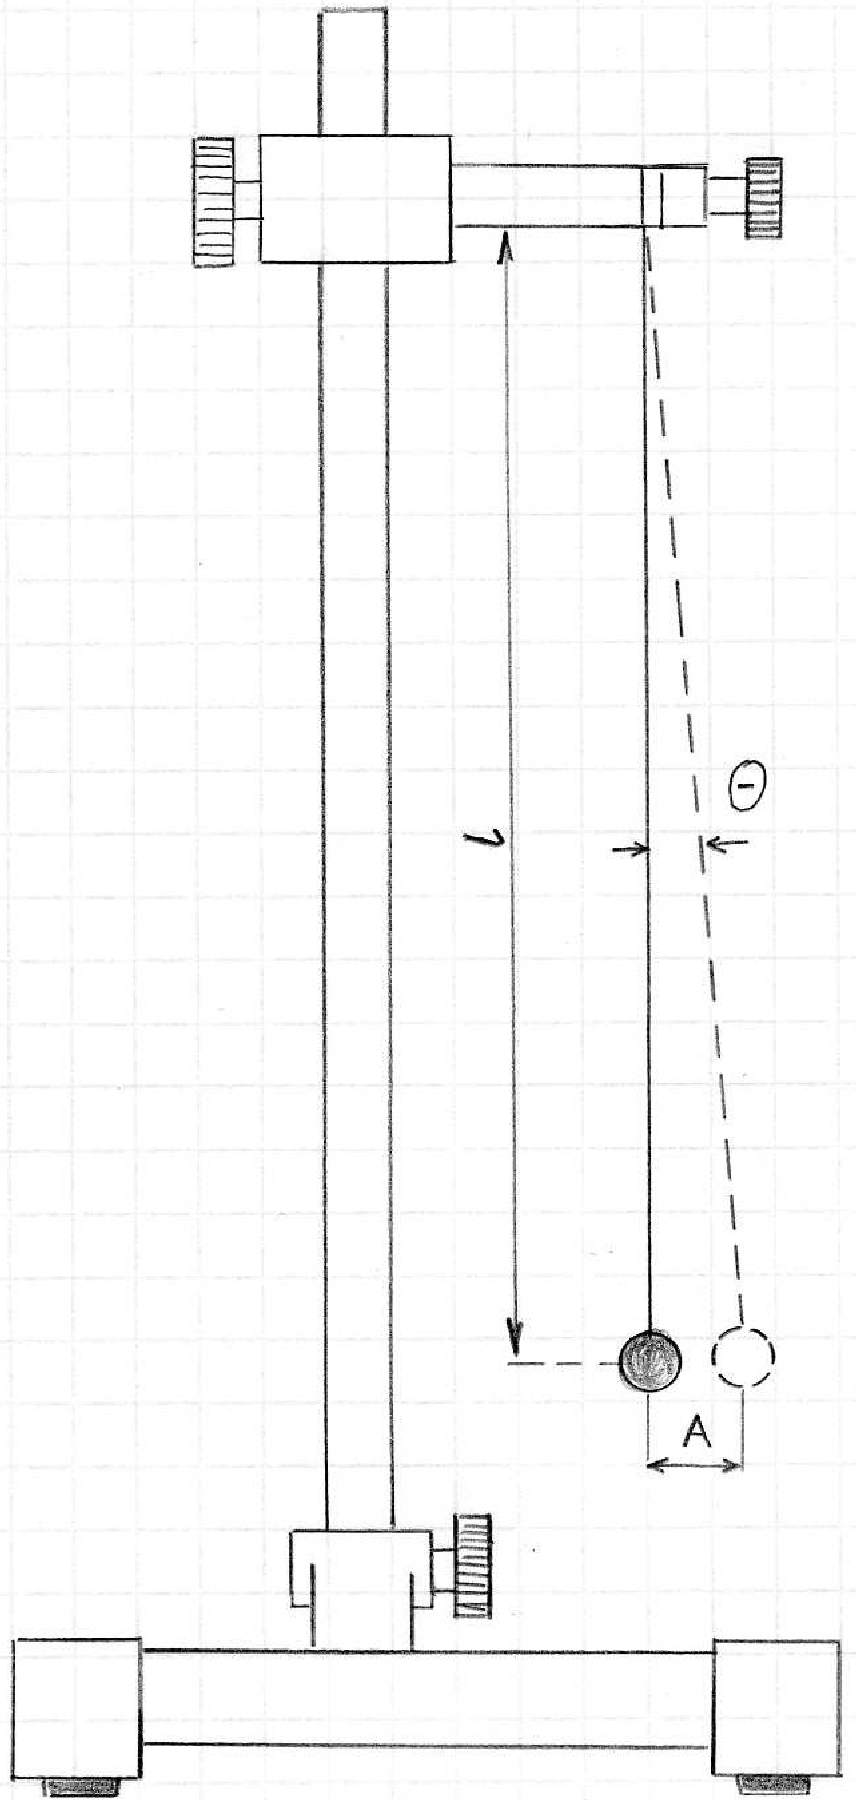
\includegraphics[width=0.18\textwidth]{./wahadlo}
\vspace*{-2.5 cm}
\end{wrapfigure}

\section{Układ pomiarowy}
Do uzyskania pomiarów niezbędny jest zestaw wahadła prostego (rysunek po prawej), sekundomierz (stoper) oraz przymiar milimetrowy (linijka).

\section{Wykonanie ćwiczenia}

Przy pomocy linijki dokonujemy pomiaru długości wahadła rozumianą jako odległość od środka ciężarka do punktu zawieszenia nici. Niewielką masę wprawiamy w ruch z małą amplitudą (nieprzekraczającą 3 stopni) i mierzymy czas wykonania się 30 pełnych okresów. Sekundomierz uruchamiamy i zatrzymujemy w tej samej fazie ruchu. Pomiar powtarzamy dziesięciokrotnie.
\newpage
W następnej kolejności chcemy zbadać pomiar zależności okresu drgań od długości wahadła, więc dziesięciokrotnie mierzymy czas wykonania się 30 pełnych okresów jak wcześniej, lecz na różnych długościach nici w zakresie od 10 cm do długości maksymalnej.
  
\section{Wyniki i ich opracowanie}

\begin{table}[ht]
\centering
\setlength{\extrarowheight}{1.5pt}
\caption{Pomiar okresu drgań przy ustalonej długości wahadła.}
Długość wahadła $l = 395 mm$, niepewność pomiarowa $u(l) = 1 mm$.
\begin{tabular}{|c|c|c|c|}
\hline
Lp. & liczba okresów $k$ & czas $t$ dla $k$ okresów w [$s$] & okres $T_{i}=t/k$ w [$s$] \\ \hline
1 & 30 & 37,37 & 1,245667\\ \hline
2 & 30 & 37,22 & 1,240667\\ \hline
3 & 30 & 37,25 & 1,241667\\ \hline
4 & 30 & 37,34 & 1,244667\\ \hline
5 & 30 & 37,06 & 1,235333\\ \hline
6 & 30 & 37,32 & 1,244000\\ \hline
7 & 30 & 37,31 & 1,243667\\ \hline
8 & 30 & 37,13 & 1,237667\\ \hline
9 & 30 & 37,47 & 1,249000\\ \hline
10 & 30 & 37,38 & 1,246000\\ \hline
\end{tabular}
\end{table}

\begin{table}[ht]
\centering
\setlength{\extrarowheight}{1.5pt}
\caption{Pomiar zależności okresu drgań od długości wahadła.}
\begin{tabular}{| @{\hspace{2mm}}c @{\hspace{2mm}}| @{\hspace{6mm}}c @{\hspace{6mm}}|@{\hspace{6mm}} c@{\hspace{6mm}}|@{\hspace{6mm}}c @{\hspace{6mm}}| @{\hspace{6mm}}c @{\hspace{6mm}}|@{\hspace{6mm}} c@{\hspace{6mm}}|}
\hline
Lp. & $l[mm]$ & $k$ & $t[s]$ & $T_{i}[s]$ & $T_{i}^{2}[s^{2}]$ \\ \hline
1 & 105 & 30 & 19,25 & 0,641667 & 0,411736\\ \hline
2 & 125 & 30 & 20,66 & 0,688667 & 0,474261\\ \hline
3 & 148 & 30 & 22,62 & 0,754000 & 0,568516\\ \hline
4 & 160 & 30 & 23,88 & 0,796000 & 0.633616\\ \hline
5 & 190 & 30 & 25,81 & 0,860333 & 0,740173\\ \hline
6 & 202 & 30 & 26,47 & 0,882333 & 0,778512\\ \hline
7 & 225 & 30 & 28,28 & 0,942667 & 0,888620\\ \hline
8 & 245 & 30 & 29,22 & 0,974000 & 0,948676\\ \hline
9 & 280 & 30 & 31,16 & 1,038667 & 1,078828\\ \hline
10 & 318 & 30 & 33,50 & 1,116667 & 1,246944\\ \hline
\end{tabular}
\end{table}

\subsection{Błąd gruby}
Nie stwierdzamy błędu grubego, żaden z wyników nie różni się znacząco od pozostałych, a przyrządy pomiarowe były umiejętnie użyte.

\subsection{Niepewność typu A - pomiar okresu}

\begin{center}
\textbf{Średnia arytmetyczna:}
\end{center}
\begin{center}
$\overline{T}=\frac{1}{n}\sum T_{\mathrm{i}}$ 
\end{center}
\begin{center} 
$\overline{T}=\dfrac{1,245667+1,245667+\cdots+1,249000+1,246000}{10}\approx1,242833s$   
\end{center}
\break
\begin{center}
\textbf{Estymator odchylenia standardowego:}
\end{center}
\begin{center}
$s_{T}=\sqrt{\frac{\sum(T_{i}-\overline{T})^{2}}{n-1}}$
\end{center}
\begin{center}
$s_{T}=\sqrt{\frac{(1,245667-1,242833)^{2}+(1,240667-1,242833)^{2}+\cdots+(1,246000-1,242833)^{2}}{10-1}}\approx0,004089s$
\end{center}
Ponieważ za wynik pomiaru przyjmujemy średnią, \textbf{niepewność pomiaru $u(T)$} utożsamiamy z~estymatorem odchylenia standardowego średniej.
\begin{center}
\textbf{Estymator odchylenia standardowego średniej:}
\end{center}
\begin{center}
$u(T)=s_{\overline{T}}=\displaystyle \frac{s_{T}}{\sqrt{n}}$
\end{center}
\begin{center}
$u(T)\approx\dfrac{0,004089s}{\sqrt{10}}\approx0,0013s$  
\end{center}

\subsection{Niepewność typu B - pomiar długości wahadła}
Długość wahadła otrzymałyśmy mierząc go przymiarem milimetrowym od środka masy ciała do punktu zawieszenia ``na oko'' -- przyjmujemy niepewność równą $u(l)=3mm$. 

\subsection{Przyspieszenie ziemskie}
Aby obliczyć przyspieszenie ziemskie korzystamy ze wzoru:
$$g=\frac{4\pi^{2}l}{\overline{T}^{2}},$$
gdzie $l$, to długość wahadła, a $\overline{T}$ to średnia arytmetyczna okresów drgań dla dziesięciu pomiarów.
$$g\approx\frac{4\pi^{2}\cdot0,395m}{(1,242833s)^{2}}\approx10,095575\dfrac{m}{s^{2}}$$

\subsection{Niepewność złożona $u_{c}(g)$}
Niepewność złożoną obliczamy korzystając z \textbf{prawa przenoszenia niepewności}.
\begin{center}
\begin{align*}
u_{c}(g)&=\sqrt{\left(\frac{\partial f}{\partial l}u(l)\right)^{2}+\left(\frac{\partial f}{\partial T}u(T)\right)^{2}}=\sqrt{\left[\frac{4\pi^{2}}{\overline{T}^{2}}u(l)\right]^{2}+\left[\frac{8\pi^{2}l}{\overline{T}^{3}}u(T)\right]^{2}}\\
&\approx\sqrt{\left[\frac{4\pi^{2}}{(1,242833s)^{2}}\cdot0,003m\right]^{2}+\left[\frac{8\pi^{2}\cdot0,395m}{(1,242833s)^{3}}\cdot0,0013s\right]^{2}}\\
&\approx0,078\dfrac{m}{s^{2}}
\end{align*}
\end{center}

Wyliczoną wartość $g$ możemy zapisać uwzględniając teraz niepewność złożoną $u_{c}(g)$:
$$g=10,100(78)\dfrac{m}{s^{2}}$$

\subsection{Niepewność rozszerzona $U(g)$}
Niepewność rozszerzoną wyrażamy jako iloczyn niepewności złożonej i bezwymiarowego współczynnika rozszerzenia $k$ (umowna wartość to $k=2$).
$$
U(g)=k \cdot u_{c}(g)\approx 2 \cdot0,078\frac{m}{s^{2}}\approx0,16\frac{m}{s^{2}}
$$
Wyliczoną wartość $g$ możemy zapisać uwzględniając teraz niepewność rozszerzoną $U(g)$:
$$g=10,10(16)\dfrac{m}{s^{2}}$$

\subsection{Porównanie z wartością tabelaryczną}
Wartość zmierzona $g_{z}$:
$$g_{z}= 10,10\dfrac{m}{s^{2}}$$
Wartość tabelaryczna $g$:
$$g= 9,811\dfrac{m}{s^{2}}$$

$$|g-g_{z}|=0,289\dfrac{m}{s^{2}}>0,16\dfrac{m}{s^{2}}$$
Wartość zmierzona nie mieści się w granicach niepewności rozszerzonej, a co za tym idzie również złożonej.

\subsection{Wykres zależności okresu od długości wahadła $T(l)$}

\begin{center}
\begin{tikzpicture}[scale=1.4]
\begin{axis}[
title={Zależność okresu od długości wahadła},
title style={text width=16em},
xlabel={Długość wahadła $l [mm]$},
ylabel={Czas jednego okresu $T [s]$},
xmin=75,xmax=325,
ymin=0.4,ymax=1.2,
legend pos=north west,
ymajorgrids=true,grid style=dashed
]
\addplot[only marks, cyan]
coordinates {
(105, 0.641666667)
(125, 0.688666667)
(148, 0.754)
(160, 0.796)
(190, 0.860333333)
(202, 0.882333333)
(225, 0.942666667)
(245, 0.974)
(280, 1.038666667)
(318, 1.116666667)
};
\end{axis}
\end{tikzpicture}
\end{center}

\subsection{Wykres zlinearyzowany $T^{2}$ w funkcji $l$} 

\begin{center}
\begin{tikzpicture}[scale=1.4]
\begin{axis}[
domain=0.125:350,samples=400,
title={Zależność kwadratu okresu od dł. wahadła},
title style={text width=18.3em},
xlabel={Długość wahadła $l [mm]$},
ylabel={Czas jednego okresu do kwadrawtu $T^{2} [s^{2}]$},
xmin=75,xmax=325,
ymin=0.4,ymax=1.3,
ymajorgrids=true,grid style=dashed
]
\addplot+[mark=none] {0.003912982*x};
\addplot[only marks, cyan]
coordinates {
(105,0.411736111)
(125,0.474261778)
(148,0.568516)
(160,0.633616)
(190,0.740173444)
(202,0.778512111)
(225,0.888620444)
(245,0.948676)
(280,1.078828444)
(318,1.246944444)
};
\end{axis}
\end{tikzpicture}
\end{center}
\subsection{Dopasowanie prostej typu $y = ax$}
Korzystając z funkcji REGLINP() w arkuszu kalkulacyjnym obliczyłyśmy współczynnik $a$ prostej $y = ax$, który wyniósł:
$$a \approx 3,912982 \dfrac{s^{2}}{m}$$
Niepewność współczynnika kierunkowego prostej:
$$u(a)\approx 0,048 \dfrac{s^{2}}{m}$$
Wyliczoną wartość $a$ możemy zapisać uwzględniając teraz niepewność $u(a)$:
$$a=3,913(48)\dfrac{s^{2}}{m}$$
Korelacja liniowa danych wyniosła $r^{2}\approx 0,998809 \pm 0,009794$, co świadczy o tym, że uzyskałyśmy dobre dopasowanie danych. Punkty układają się na lub bardzo blisko linii prostej $y=3,913x$, co widać to także na powyższym wykresie.

\subsection{Wartość przyspieszenia ziemskiego z otrzymanej wartości współczynnika nachylenia $a =\dfrac{4\pi^{2}}{g}$}
Przekształcając wzór do postaci:
$$g = \dfrac{4\pi^{2}}{a}$$
oraz podstawiając współczynnik kierunkowy $a$ wyliczony w poprzednim podpunkcie otrzymujemy:
$$g \approx \dfrac{4\pi^{2}}{3,912982\dfrac{s^{2}}{m}} \approx 10,089088\dfrac{m}{s^{2}}$$

\subsection{Niepewność $u(g)$ na podstawie uzyskanej z dopasowania niepewności $u(a)$}
Wyprowadzając wzór i podstawiając otrzymane wcześniej wartości $a$ oraz $u(a)$ otrzymujemy: 
$$u(g)=\sqrt{\left[\frac{\partial g}{\partial a}u(a)\right]^{2}}=\left|\frac{\partial g}{\partial a}u(a)\right|=\left|\frac{\partial\frac{4\pi^{2}}{a}}{\partial a}u(a)\right|=\left|\frac{-4\pi^{2}}{a^{2}}u(a)\right|$$
$$u(g)\approx\left|\frac{-4\pi^{2}}{ \left(3,913 \dfrac{s^{2}}{m}\right)^{2}}0,048 \dfrac{s^{2}}{m}\right| \approx 0,12\dfrac{m}{s^{2}}$$
Wyliczoną wartość $g$ możemy zapisać uwzględniając teraz niepewność $u(g)$ na podstawie uzyskanej z dopasowania niepewności $u(a)$:
$$g=10,10(12)\dfrac{m}{s^{2}}$$

\subsection{Porównanie z wartością tabelaryczną}
Wartość zmierzona $g_{z}$:
$$g_{z}= 10,10\dfrac{m}{s^{2}}$$
Wartość tabelaryczna $g$:
$$g= 9,811\dfrac{m}{s^{2}}$$

$$|g-g_{z}|=0,289\dfrac{m}{s^{2}}> 0,12\dfrac{m}{s^{2}}$$
Wartość zmierzona nie mieści się w granicach niepewności $u(g)$ na podstawie uzyskanej z dopasowania niepewności $u(a)$.

\section{Wnioski}
\begin{itemize}
\item Otrzymane wartości nie zgadzają się z wartościami tabelarycznymi i nie mieszczą się również w zakresie niepewności. Przyczyną błędu mogą być niewystarczająco dokładne przyrządy pomiarowe, niewykryty wcześniej błąd systematyczny np. związany z uruchamianiem i zatrzymywaniem stopera lub zbyt duża amplituda z jaką wahał się ciężarek.  
\item Różnica otrzymanego przez nas przyspieszenia i standardowego przyspieszenia dla Krakowa $g=9,811\dfrac{m}{s^{2}}$ nie jest jednak tak wielka, więc można stwierdzić, że błędu grubego nie popełniono.
\item Wraz z wydłużeniem nici, na której zawieszony jest ciężarek rośnie też okres wahadła. Tak jak zostało to przedstawione na wykresie w podpunkcie 5.8, zależność kwadratu okresu od długości wahadła jest zależnością proporcjonalną.
\end{itemize}
\end{document}